%%%%%%%%%%%%%%%%%%%%%%%%%%%%%%%%%%%%%%%%%%%%%%%%%%%%%%%%%%%%%%%%%
% Dissertacao de Mestrado / Dept Fisica, CFM, UFSC              %
% Andre@UFSC - 2011                                             %
%%%%%%%%%%%%%%%%%%%%%%%%%%%%%%%%%%%%%%%%%%%%%%%%%%%%%%%%%%%%%%%%%

%:::::::::::::::::::::::::::::::::::::::::::::::::::::::::::::::%
%                                                               %
%                          Capítulo 3                           %
%                                                               %
%:::::::::::::::::::::::::::::::::::::::::::::::::::::::::::::::%

%***************************************************************%
%                                                               %
%                         Crossmatch                            %
%                                                               %
%***************************************************************%

\chapter{Estendendo a base de dados \SDSS/\STARLIGHT para o ultravioleta}
\label{sec:Crossmatch}


%***************************************************************%
%                                                               %
%              Crossmatch - Banco de dados do SDSS              %
%                                                               %
%***************************************************************%

\section{Banco de dados do \SDSS}

Um dos maiores responsáveis pela promoção do uso de bancos de dados relacionais
na astronomia é o projeto {\em Sloan Digital Sky Survey} (\SDSS). Inicialmente o
\SDSS utilizou um {\em sistema de gerenciamento de banco de dados orientado a
objetos} \citep[OODBMS;][]{Maier1986}. Após pouco mais de um ano a abordagem se
mostrou inadequada: entre os principais problemas, uma linguagem de {\em query}
inadequada e performance ruim. O motivo, segundo \citet{Thakar2004}, foi a
incapacidade da empresa desenvolvedora do OODBMS em prover novas funcionalidades
requisitadas pelo projeto e correção de {\em bugs}, bem como em acompanhar o
crescimento da performance do {\em hardware}.

\subsection{Migração de OODBMS para RDBMS}
\label{sec:CrossMatch:SDSS:MigracaoRDBMS}

Todo o banco de dados do \SDSS foi migrado para um {\em sistema de gerenciamento
de banco de dados relacional} \citep[RDBMS;][]{Codd1970} num esforço guiado por
\citeauthor{Thakar2004}. RDBMS pode ser considerado o padrão da indústria.
Praticamente todas as linguagens de programação tem bibliotecas de interface às
implementações de RDBMS comerciais mais comuns (Oracle, IBM e Microsoft,
Postgres). Há uma diversidade de ferramentas para desenvolvimento e
gerenciamento de RDBMS. E talvez o maior benefício de todos, o acesso aos dados
é feito utilizando uma linguagem padronizada: {\em Simple Query Language}, ou
simplesmente SQL \citep{Chamberlin1974}. A migração dos dados do \SDSS para um
RDBMS comercial implicou num aumento significativo da performance do acesso aos
dados, e resultou no desenvolvimento do {\em SkyServer}\footnote{\SDSS
SkyServer: \url{http://skyserver.sdss.org/}}. O servidor de banco de dados
escolhido pelo \SDSS foi o {\em Microsoft SQL Server}.

A comparação entre OODBMS e RDBMS no caso particular do \SDSS não implica
necessariamente a superioridade do segundo em relação ao primeiro. Tanto a
abordagem orientada a objetos quanto a abordagem relacional tem suas vantagens e
desvantagens. O estudo de caso do \SDSS é apenas uma evidência anedótica em
favor do uso de bancos de dados relacionais. No entanto, para aplicações
semelhantes ao \SDSS -- {\em surveys} astronômicos com volumes imensos de dados
-- vale a pena apostar no sucesso dos RDBMS.

\subsection{{\em SkyServer}}
\label{sec:CrossMatch:SDSS:SkyServer}

O {\em SkyServer} é um {\em website} (figura \ref{fig:TelaDoSkyServer}) que
provê acesso aos dados armazenados no banco de dados do \SDSS
\citep{Szalay2002}. O acesso mais simples pode ser feito através de um atlas de
locais famosos ({\em famous places}), que mostra imagens coloridas de objetos
celestes conhecidos. Há formulários para buscas mais sérias, gerando coleções de
imagens, espectros e tabelas de dados. No {\em SkyServer} é possível fazer
buscas avançadas utilizando SQL, embora haja limites de tempo de execução e de
quantidade de objetos retornados. Esta limitação é contornada através do sistema
{\em CasJobs}, que é tratado na seção \ref{sec:CrossMatch:SDSS:CasJobs}.

É importante ressaltar que é possível (de fato, a equipe do \SDSS encoraja)
criar {\em mirrors}\footnote{{\em Mirror}: Espelho, em inglês. Clone de um {\em
website}.} do {\em SkyServer}. Tanto o banco de dados do \SDSS quanto o código
fonte do {\em SkyServer} estão disponível no próprio {\em website} do {\em
SkyServer}. Temos um clone do banco de dados do {\em Data Release} 8 do \SDSS no
servidor {\em CasJobs} do \starlight \footnote{{\em CasJobs} do \starlight:
\url{http://casjobs.starlight.ufsc.br/casjobs/}}.

\begin{figure}
	\includegraphics[width=1.0\columnwidth]{figuras/skyserver.eps}
	\caption[Telas do {\em SkyServer}.]
	{Telas do {\em SkyServer}. À esquerda, formulário para submeter uma {\em
	query} SQL. À direita, ferramenta {\em Explore} mostrando a galáxia NGC 799.}
	\label{fig:TelaDoSkyServer}
\end{figure}

\subsection{{\em CasJobs}}
\label{sec:CrossMatch:SDSS:CasJobs}

O {\em Catalog Archive Server Jobs} ({\em CasJobs}) é um serviço online
desenvolvido pela equipe do \SDSS para expandir a capacidade do {\em SkyServer}
\citep{Li2008}. Nele o usuário pode executar consultas SQL no banco de dados do
\SDSS da mesma forma que no {\em SkyServer}. Porém, além de consultas rápidas, é
possível agendar a execução de consultas mais longas. O {\em CasJobs} gerencia
estas consultas agendadas numa fila de execução, de modo a não sobrecarregar a
rede ou os servidores de banco de dados. Cada usuário possui seu próprio banco
de dados, chamado {\em MyDB}. Pode-se importar tabelas para o {\em MyDB} para
utilizar em {\em queries} correlacionando com os dados presentes no {\em
CasJobs}. O {\em MyDB} serve como armazenamento de tabelas do usuário, e há
mecanismos para exportar estas tabelas para arquivos nos formatos FITS, CSV, XML
e VOTable. Estes arquivos podem ser lidos por programas de análise de dados como
o {\em TopCat}\footnote{{\em TopCat} é um visualizador gráfico interativo e
editor de dados tabulares usado em astronomia. Ver
\url{http://www.star.bris.ac.uk/~mbt/topcat/}.}, ou mesmo importados para outros
bancos de dados.

\begin{figure}
	\includegraphics[width=0.7\columnwidth]{figuras/casjobs.eps}
	\caption[Tela do {\em CasJobs}.]
	{Tela do {\em CasJobs}. Resultado da {\em query} buscando o {\em redshift}, a
	magnitude na banda $g$, a cor $g-r$ e uma amostra da imagem de objetos com
	espectroscopia.}
	\label{fig:CasJobs}
\end{figure}

É possível utilizar o {\em CasJobs} para acessar virtualmente qualquer banco de
dados. No momento, o Grupo de Astrofísica da UFSC possui um servidor {\em
CasJobs} com bancos de dados do \starlight, \SDSS DR8, GalaxyZoo
\citep{Lintott2008}, e uma amostra do \galex e um catálogo de {\em redshifts}
fotométricos \citep{OMill2011}. O {\em CasJobs} também foi adotado por outros
projetos como o \galex, {\em Kepler}\footnote{{\em Kepler CasJobs}:
\url{http://mastweb.stsci.edu/kplrcasjobs/}} e o {\em Palomar Quest
}\footnote{{\em Palomar Quest CasJobs}:
\url{http://webvoy.cacr.caltech.edu/CasJobs/}} \citep{Djorgovski2008}.

A figura \ref{fig:CasJobs} mostra uma tela típica de uma sessão no {\em
CasJobs}.


%***************************************************************%
%                                                               %
%          Crossmatch - Banco de dados do STARLIGHT             %
%                                                               %
%***************************************************************%

\section{Banco de dados do \STARLIGHT}

O \starlight é um código de síntese espectral \citep{CidFernandes2005}. O
programa é executado uma vez para cada galáxia do \SDSS, recebendo seu espectro
como um arquivo texto. Ele usa uma biblioteca de espectros SSPs com diferentes
idades e metalicidades como uma base do espaço de espectros galáticos possíveis.
De forma simplificada, o que o \starlight faz é encontrar as frações de massa e
luz correspondente a cada elemento da base, ou seja, cada SSP. Analisando as
relações entre os componentes determinados pela síntese, o programa determina
diversas propriedades físicas da galáxia, como a massa estelar total, a massa
separada por idade, metalicidade média, quantidade de poeira e dispersão de
velocidade, para citar apenas algumas. Quase um milhão de espectros foram
analisados, e o resultado da síntese foi armazenado em arquivos texto.

Somente os componentes estelares do espectro são obtidos desta forma. Subtraindo
o espectro sintetizado de luz estelar é possível medir as linhas de emissão do
espectro. Esta é uma etapa de pós-processamento, que gera um catálogo
complementar de linhas de emissão.

\subsection{Importação para o RDBMS}

Os arquivos da síntese gerados pelo \starlight ocupam quase trezentos gigabytes.
Mesmo o catálogo de propriedades físicas das galáxias, sozinho, ocupa mais de um
gigabyte. Embora seja um volume razoavelmente grande de dados, é possível
trabalhar com esta quantidade de dados num computador atual\footnote{Quando esta
dissertação foi escrita, era bastante comum comprar um computador pessoal novo
com 4 gigabytes de memória RAM ou mais.}. A transferência de arquivos com
tamanho da ordem de gigabytes pela internet também também é lugar-comum
atualmente. Poderia-se argumentar que distribuir os dados neste formato seja a
forma mais adequada.

Entretanto, deve-se admitir que uma das maiores razões para o sucesso do {\em
CasJobs} em prover acesso aos dados o \SDSS não é o tamanho da base de dados, e
sim a facilidade com que o usuário pode acessar os dados e filtrar somente o que
lhe for conveniente. Além disso, manter a base de dados num local central
permite que sejam feitas correções e revisões, o que implicaria normalmente numa
nova transferência caso cada usuário tivesse a sua cópia local.

O {\em CasJobs} requer um servidor rodando {\em Windows Server} com {\em
Internet Information Services} (IIS) e {\em Microsoft SQL Server} (MSSQL). A
instalação do {\em CasJobs} está documentada no {\em website} do {\em SkyServer}
(ver seção \ref{sec:CrossMatch:SDSS:SkyServer}). Com um servidor {\em CasJobs},
o trabalho consiste em importar os dados em arquivos texto para um banco de
dados no MSSQL. A ferramenta principal para a manipulação dos bancos de dados no
MSSQL é o {\em Microsoft SQL Server Management Studio}. Nele há um assistente
para importação de dados baseado no {\em SQL Server Integrated Services} (SSIS).
A importação das tabelas de propriedades físicas do \starlight foi feita
rapidamente através desta ferramenta. Entretanto, foi necessário
normalizar\footnote{A normalização consiste em decompor uma tabela em tabelas
menores (com menos campos) de forma que elas fiquem melhor estruturadas. No caso
das linhas de emissão, a tabela passa de ``todas as linhas de um dado objeto num
único registro'' para ``uma linha para cada registro''. No primeiro caso,
adicionar um novo tipo de linha de emissão implicaria em mudar a estrutura da
tabela, o que é evitado utilizando a segunda abordagem.} a tabela de linhas de
emissão para facilitar a inclusão de novas linhas no futuro.

\subsection{Estrutura do banco de dados}
\label{sec:Crossmatch:EstruturaBDStarlight}

O esquema do banco de dados do \starlight pode ser visto na figura
\ref{fig:EsquemaBDStarlight}. Os dados observacionais obtidos do \SDSS estão na
tabela \texttt{observational\_params}. Estes dados, junto com os parâmetros de
entrada da síntese (tabela \texttt{synthesis\_params}), foram usados como
parâmetros para a obtenção das propriedades físicas das galáxias, armazenadas na
tabela \texttt{synthesis\_results}. Estas tabelas estão ligadas através dos
campos \texttt{SpecObjID} e \texttt{SynID}. As linhas de emissão estão
armazenadas na tabela \texttt{el\_fit}, ligada à \texttt{synthesis\_results}
através do campo \texttt{SynID}. A definição das linhas (comprimento de onda e
faixas contínuo usadas na medida) está contida na tabela \texttt{cfg\_el\_fit}.
As tabelas referentes ao \galex são explicadas na seção
\ref{sec:Crossmatch:DefAmostras:IdSDSSGalex}.

\begin{figure}
	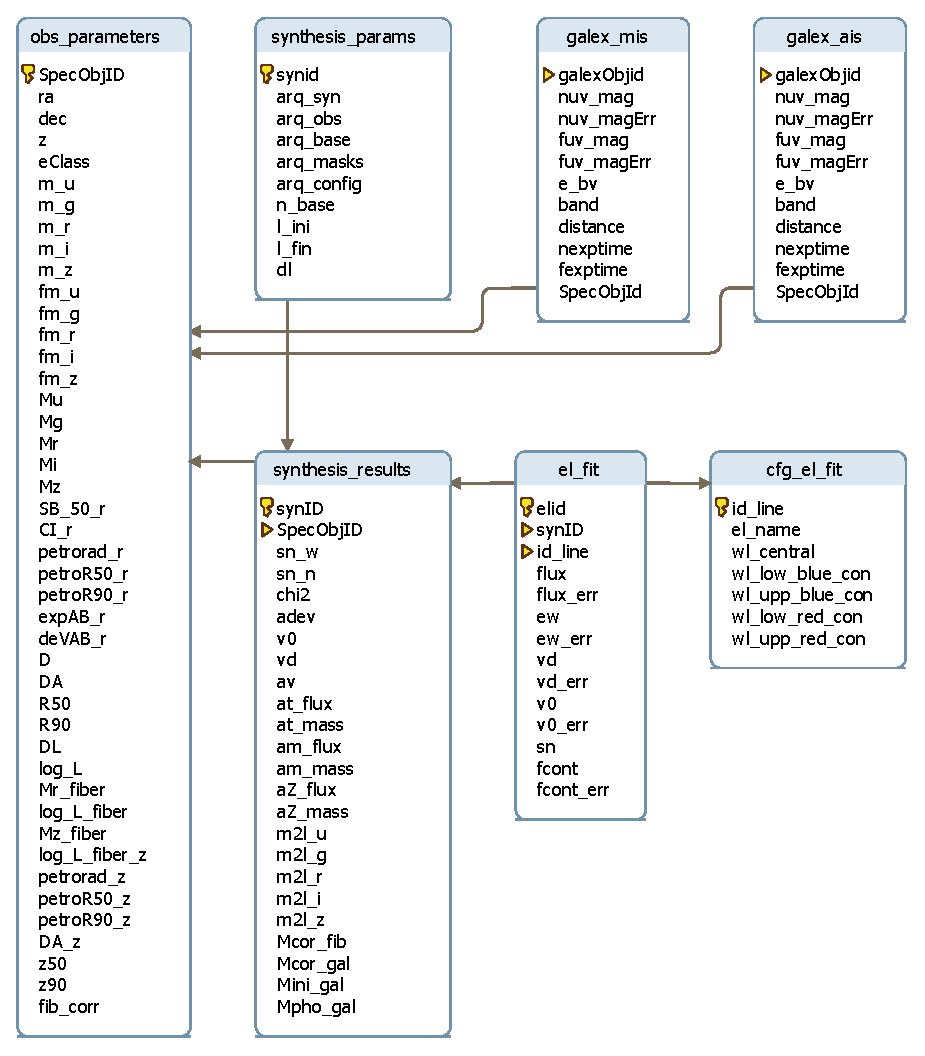
\includegraphics{figuras/starlight-schema.eps}
	\caption[Esquema do banco de dados do \starlight.]
	{Esquema do banco de dados do \starlight. As linhas indicam chaves
	estrangeiras, relacionando dois campos de duas tabelas diferentes.}
	\label{fig:EsquemaBDStarlight}
\end{figure}

\subsection{Amostra do \STARLIGHT}
\label{sec:Crossmatch:AmostraStarlight}

A amostra de galáxias do \starlight contém $926246$ espectros do \SDSS DR7
\citep{Abazajian2009}. A identificação de cada espectro é feita através de um
tripleto: a data juliana média da observação (\texttt{MJD}, {\em Mean Julian
Date}), a identificação da placa de suporte das fibras ópticas (\texttt{Plate})
e a identificação da fibra utilizada para a obtenção do espectro
(\texttt{FiberID}). Este tripleto (\texttt{MJD}, \texttt{Plate},
\texttt{FiberID}) identifica unicamente um espectro. Porém, é mais conveniente
(e eficiente) ter um identificador único (uma chave primária\footnote{Chave
primária é um conjunto de um ou mais campos tais que a combinação de todos os
campos da chave não se repete.}) para os registros num banco de dados. No caso
do \SDSS, a tabela de espectros (\texttt{SpecObjAll}) tem um identificador
chamado \texttt{SpecObjID}.

Além de espectros, o banco de dados do \SDSS contém fotometria de $1/4$ do céu.
Os objetos com dados de fotometria também tem um identificador único,
\texttt{ObjID}. Existe uma coluna na tabela de espectros chamada
\texttt{BestObjID}, que aponta para o registro de fotometria (tabela {\tt
PhotoObjAll}) mais provável para cada espectro. É importante salientar que nem
todo espectro tem um \texttt{BestObjID} definido.

A tabela de índices da amostra de galáxias do \starlight contém inicialmente os
tripletos [\texttt{MJD}, \texttt{Plate}, \texttt{FiberID}]. Esta tabela é
importada para o ambiente {CasJobs} do \SDSS DR7\footnote{{\em CasJobs} \SDSS
DR7 - \url{http://casjobs.sdss.org/CasJobs/}}. Através da execução da {\em
query} da figura \ref{fig:QueryAtualizaObjIds} a tabela tem os valores de
\texttt{SpecObjID} e \texttt{BestObjID} preenchida. Entre os objetos na amostra
do \starlight, $622$ objetos não possuem um valor de \texttt{BestObjID}
definido, ou seja, não foi possível encontrar a sua contrapartida fotométrica.


%***************************************************************%
%                                                               %
%                   Crossmatch - SDSS X GALEX                   %
%                                                               %
%***************************************************************%

\section{Identificação cruzada entre \SDSS e \galex}
\label{sec:Crossmatch:SDSSGalex}

A identificação cruzada ({\em crossmatch}) de objetos em {\em surveys}
diferentes é um problema razoavelmente complicado. A cobertura do céu de cada
{\em survey} em geral não é a mesma. Por outro lado, os objetos presentes em um
{\em survey} podem não ter sido detectados no outro. A probabilidade de duas
fontes em catálogos diferentes corresponderem a um mesmo objeto pode ser
calculada como função da separação entre elas e a precisão astrométrica das
medidas \citep{Budavari2008}.

\citet{Budavari2009} aplicam este método probabilístico ao \SDSS e ao \galex. O
{\em crossmatch} espacial é feito dentro de um RDMS (MSSQL, o mesmo usado no
{\em CasJobs}), utilizando técnicas avançadas de indexação \citep[ {\em
Hierarchic Triangular Mesh}]{Kunszt2000}. A tabela resultante é uma relação
``muitos para muitos'', onde a maioria dos objetos \galex tem apenas um objeto
\SDSS associado, mas outras associações podem ocorrer. Um exemplo onde pode
ocorrer uma associação ``um para muitos'' é o caso onde existe uma fonte fraca
em UV (presente no \SDSS mas não detectada pelo \galex) próxima a uma fonte
presente tanto no UV quanto no óptico. O algoritmo irá apontar estes dois
objetos no \SDSS como candidatos a serem a contrapartida óptica do objeto
detectado no \galex. O caso inverso implicaria numa associação ``muitos para
um''. Nas tabelas \ref{tab:SDSSxGalexMatchesAIS} e
\ref{tab:SDSSxGalexMatchesMIS} há a quantidade de identificações para cada tipo
de associação, referentes aos {\em surveys} AIS e MIS, respectivamente. Os
valores foram determinados para o {\em crossmatch} entre \SDSS DR7 e \galex GR6,
disponível no {\em CasJobs} do \galex\footnote{{\em CasJobs} \galex:
\url{http://galex.stsci.edu/casjobs/}}). O artigo citado acima mostra a mesma
tabela, com os resultados para dados do \SDSS DR6 e \galex GR3. A técnica
utilizada por \citeauthor{Budavari2009} agora faz parte do {\em pipeline} do
\galex. A distribuição do {\em CasJobs} inclui as ferramentas necessárias para
fazer o {\em crossmatch} espacial entre bancos de dados.

\begin{table}
	\caption[Identificações entre \SDSS DR7 e {\em survey} AIS do \galex GR6.]
	{Número de identificações entre \SDSS DR7 e {\em survey} AIS do \galex GR6, por
	associação. A lista foi gerada pela {\em query} mostrada na figura
	\ref{fig:QueryIDGalexSDSS}.}
	\setlength{\tabcolsep}{1cm}
	\begin{tabular}{r r r r}
		\galex &          \multicolumn{3}{c}{\SDSS} \\
		\midrule
		       &              1 &             2 &        Muitos \\
		1      & $15\,267\,818$ & $9\,150\,919$ & $4\,623\,197$ \\
		2      &  $4\,524\,337$ & $2\,504\,786$ & $1\,162\,463$ \\
		Muitos &     $770\,645$ &    $426\,691$ &    $184\,680$ \\
	\end{tabular}
	\label{tab:SDSSxGalexMatchesAIS}
\end{table}

\begin{table}
	\caption[Identificações entre \SDSS DR7 e {\em survey} AIS do \galex GR6.]
	{Número de identificações entre \SDSS DR7 e {\em survey} MIS do \galex GR6, por
	associação. A lista foi gerada pela {\em query} mostrada na figura
	\ref{fig:QueryIDGalexSDSS}.}
	\setlength{\tabcolsep}{1cm}
	\begin{tabular}{r r r r}
		\galex &         \multicolumn{3}{c}{\SDSS} \\
		\midrule
		       &             1 &             2 &        Muitos \\
		1      & $8\,201\,735$ & $5\,923\,551$ & $3\,775\,187$ \\
		2      & $2\,120\,174$ & $1\,580\,701$ &    $984\,067$ \\
		Muitos &    $276\,447$ &    $234\,016$ &    $150\,894$ \\
	\end{tabular}
	\label{tab:SDSSxGalexMatchesMIS}
\end{table}


%***************************************************************%
%                                                               %
%     Crossmatch - Obtendo dados UV para a amostra STARLIGHT    %
%                                                               %
%***************************************************************%

\section{Obtendo dados UV para a amostra \STARLIGHT}
\label{sec:Crossmatch:DefAmostras}

\subsection{Relação de {\em crossmatch} entre \SDSS e \galex}
\label{sec:Crossmatch:DefAmostras:IdSDSSGalex}

Como comentado na seção \ref{sec:Crossmatch:SDSSGalex}, no banco de dados do
\galex há uma tabela de {\em crossmatch} entre os objetos do \galex e os seus
correspondentes ópticos no catálogo do \SDSS, chamada \texttt{xSDSSDR7}. A
descrição completa dos campos pode ser vista na tabela \ref{tab:CamposXSDSSDR7}.
Dado que a identificação não é necessariamente unívoca, existem informações
extras nesta tabela a fim de facilitar a seleção dos melhores candidatos: {\tt
DistanceRank} e \texttt{MultipleMatchCount}.

A identificação cruzada também é feita na direção oposta. Dado um objeto do
\SDSS, foram encontrados os objetos do \galex candidatos. Para um par [{\tt
ObjID}, \texttt{SDSSObjID}], há também os campos \texttt{ReverseDistanceRank} e
{\tt ReverseMultipleMatchCount}.

\begin{table}
	\caption[Descrição dos campos da tabela \texttt{xSDSSDR7}.]
	{Descrição dos campos da tabela \texttt{xSDSSDR7}.}
	\begin{tabular}{l p{8cm}}
		Campo & Descrição\\
		\midrule
		\texttt{ObjID} &
		Identificador único de objeto do \galex.
		\\
		\texttt{SDSSObjID} &
		Identificador único do \SDSS.
		\\
		\texttt{Distance} &
		Separação angular em segundos de arco.
		\\
		\texttt{DistanceRank} &
		Um número inteiro, onde o valor $1$ indica que o objeto do \galex é o
		mais próximo do objeto \SDSS, o valor $2$ indica que ele é o segundo mais
		próximo, etc.
		\\
		\texttt{ReverseDistanceRank} &
		Um número inteiro, onde o valor $1$ indica que o objeto do \SDSS é o mais
		próximo do objeto \galex, o valor $2$ indica que ele é o segundo mais
		próximo, etc.
		\\
		\texttt{MultipleMatchCount} &
		Um número inteiro indicando quantos objetos \SDSS foram encontrados para o
		objeto \galex dentro do raio de busca.
		\\
		\texttt{ReverseMultipleMatchCount} &
		Um número inteiro indicando quantos objetos \galex foram encontrados para o
		objeto \SDSS dentro do raio de busca.
		\\
	\end{tabular}
	\label{tab:CamposXSDSSDR7}
\end{table}

\subsection{Dados UV}

A amostra do \starlight descrita na seção \ref{sec:Crossmatch:AmostraStarlight}
contém o identificador do catálogo de fotometria do \SDSS. Este identificador é
o mesmo utilizado na tabela \texttt{XSDSSDR7}. A {\em query} da figura
\ref{fig:QueryMatchAIS} preenche a tabela chamada \texttt{galex\_ais} com todos
os objetos da amostra do \starlight, junto com suas respectivas magnitudes NUV
(\texttt{FUV\_mag}) e FUV (\texttt{NUV\_mag}), o erro na medida das magnitudes
({\tt FUV\_magErr} e \texttt{NUV\_magErr}), o tempo de exposição em cada filtro
({\tt fexptime} e \texttt{nexptime}), o excesso de cor $E(B-V)$ (\texttt{e\_bv},
ver seção \ref{sec:Crossmatch:DefAmostras:Correcoes}) e a distância entre a
detecção do objeto no \galex e no \SDSS (\texttt{distance}). Esta tabela é
esparsamente populada, com um registro para cada objeto do \starlight, e os
dados UV preenchidos somente para os objetos com identificação positiva. Caso o
objeto não tenha um correspondente \galex, os valores serão nulos\footnote{Numa
tabela, quando um campo de um registro não possui valor definido, seu valor é
dito ``nulo''. Em SQL, a palavra-chave que representa um valor nulo é ``{\em
null}''.}. De forma similar, os dados UV para o {\em survey} MIS foram
armazenados na tabela \texttt{galex\_mis}. Estas tabelas podem ser vistas no
contexto do banco de dados do \starlight na seção
\ref{sec:Crossmatch:EstruturaBDStarlight}.

Foram escolhidas somente identificações cruzadas do tipo um-para-um, ou seja,
registros com \texttt{multipleMatchCount} e \texttt{reverseMultipleMatchCount}
iguais a 1. Em situações diferentes desta, caso houvesse mais de um candidato
para uma mesma detecção, seria necessária uma análise mais detalhada. Desta
forma, optou-se por uma confiabilidade maior nos dados utilizando apenas
identificações unívocas, em troca de uma amostra menor.

Outro artefato importante é que somente um objeto \galex foi escolhido para cada
objeto do catálogo do \starlight, independente do {\em survey} utilizado. Se
existe um correspondente AIS e outro MIS para o mesmo objeto da amostra, apenas
o mais próximo é considerado. Nos campos onde os dois {surveys} se sobrepõem, há
uma maior quantidade de objetos no MIS do que no AIS, devido ao maior tempo de
exposição no MIS. Assim, nesses campos, os objetos do MIS têm maior chance de
estar mais próximos ao objeto do \SDSS. Isto também não é um problema muito
grave para o AIS, já que a sua cobertura do céu é muito maior do que a do MIS. A
fração exata de objetos perdidos em cada caso ainda precisa ser determinada.
Esta correção será feita futuramente numa revisão do catálogo.

No total foram obtidas $173\,218$ detecções no AIS e $41\,274$ no MIS. Nem todos
os objetos tiveram detecção simultânea nas bandas FUV e NUV. A tabela
\ref{tab:DetBanda} lista a quantidade de objetos que possuem valor definido de
acordo com cada banda UV. Alguns objetos podem ser muito fracos em FUV. Isto
combinado com a baixa eficiência do filtro (figura \ref{fig:GalexFilters}) e do
detetor podem fazer com que a contagem de fótons deste objeto seja muito baixa,
ficando abaixo do nível limite de sinal-ruído do {\em survey}.

\begin{table}
	\caption[Número de detecções por banda no catálogo UV do \STARLIGHT.]
	{Número de detecções por banda no catálogo UV do \starlight. Nas linhas FUV e
	NUV, é listada a quantidade de objetos com detecção para os {\em
	surveys} AIS e MIS nas bandas FUV e NUV, respectivamente. A linha FUV+NUV
	lista a quantidade de objetos com detecção simultânea em FUV e NUV. A figura
	\ref{fig:QueryListaPorBandaSurvey} contém a {\em query} que gera esta lista.}
	\setlength{\tabcolsep}{1cm}
	\begin{tabular}{l r r}
		Banda   &        AIS &       MIS \\
		\midrule
		FUV     & $107\,902$ & $13\,685$ \\
		NUV     & $168\,126$ & $38\,828$ \\
		FUV+NUV & $102\,811$ & $11\,239$ \\
	\end{tabular}
	\label{tab:DetBanda}
\end{table}

\subsection{Correções aplicadas à fotometria UV}
\label{sec:Crossmatch:DefAmostras:Correcoes}

O catálogo do \galex fornece a fotometria NUV e FUV dos objetos em magnitude
aparente, sem qualquer correção a não ser por fatores instrumentais. Para que as
galáxias possam ser analisadas de forma adequada, algumas correções precisam ser
feitas.

A luz proveniente de outras galáxias sofre extinção causada por poeira dentro da
nossa própria Galáxia\footnote{A existência de poeira na Via Láctea pode ser
notada facilmente a olho nu em uma noite sem lua -- e bem longe da luz da
cidade!}. Esta extinção depende da direção de onde vem a luz, e a sua influência
depende do comprimento de onda. O efeito final, em geral, é o avermelhamento do
espectro. O excesso de cor $E(B-V)$ representa quantitativamente este
avermelhamento.

O catálogo do \galex provê os valores de excesso de cor $E(B-V)$ das galáxias
com base nos mapas de extinção interestelar de \citet{Schlegel1998}. A correção
é feita usando o modelo de extinção CCM \citep[equações 4a e 4b]{Cardelli1989}.
Para um comprimento de onda $\lambda$ qualquer, a extinção absoluta (em
magnitudes) é dada por
\begin{eqnarray*}
	A_\lambda &=& R_V\,E(B-V)\,a(x) + E(B-V)\,b(x), \\
	x &=& \frac{10000\text{\AA}}{\lambda}.
\end{eqnarray*}
No caso das bandas FUV ($\lambda_{eff}=1528\text{\AA}$) e NUV
($\lambda_{eff}=1528\text{\AA}$),
\begin{eqnarray*}
	x_{FUV} &=& 6,54\\
	x_{NUV} &=& 4,40
\end{eqnarray*}
com os coeficientes $a(x)$ e $b(x)$ dados por
\begin{eqnarray*}
	a(x) &=& 1,752 - 0,326x - 0,104/[(x-4,67)^2 + 0,341] + F_a(x) \\
	b(x) &=& -3,090 + 1,825x + 1,206/[(x-4,62)^2 + 0,263] + F_b(x) \\
	\\
	F_a(x_{FUV}) &=& F_b(x_{FUV}) = 0 \\
	F_a(x_{NUV}) &=& -0,04473(x_{NUV}-5,9)^2 - 0,09779(x_{NUV}-5,9)^3 \\
	F_b(x_{NUV}) &=& 0,2130(x_{NUV}-5,9)^2 + 0,1207(x_{NUV}-5,9)^3.
\end{eqnarray*}
Usando $R_V=3,1$, a extinção nas bandas FUV e NUV em função do excesso de cor
$E(B-V)$ é dada por
\begin{eqnarray*}
	A_{FUV} &=& 8,15\,E(B-V) \\
	A_{NUV} &=& 9,17\,E(B-V).
\end{eqnarray*}
Esta correção é então aplicada às magnitudes do catálogo.

Foi aplicada também a correção $k(z)$ devida ao {\em redshift}, e a magnitude
foi transformada em magnitude absoluta, utilizando o código \textsc{kcorrect}
(v4\_2) de \citet{Blanton2007}.


%***************************************************************%
%                                                               %
%        Crossmatch - Definição da amostra STARLIGHT+UV         %
%                                                               %
%***************************************************************%

\section{Definição da amostra \STARLIGHTUV}
\label{sec:Crossmatch:DefAmostras:StarlightUV}

A {\em query} mostrada na figura \ref{fig:QuerySampleAIS} monta a amostra a ser
utilizada no capítulo seguinte. As colunas selecionadas são as magnitudes
$ugriz$ do \SDSS, a magnitude NUV do \galex e algumas propriedades físicas das
galáxias (tabela \ref{tab:ParamFisicos}). Foram selecionadas também a largura
equivalente e o fluxo das linhas de emissão \Halpha, \Hbeta, \OIII e \NII.

\begin{table}
	\caption[Propriedades físicas das galáxias utilizados na amostra.]
	{Propriedades físicas das galáxias, obtidos do \starlight.}
	\begin{tabular}{l l}
		Coluna & Descrição \\
		\midrule
		\texttt{mcor\_gal} & Logaritmo da massa estelar \\
		\texttt{at\_flux}  & Logaritmo da idade média ponderada em fluxo \\
		\texttt{at\_mass}  & Logaritmo da idade média ponderada em massa \\
		\texttt{am\_flux}  & Metalicidade média ponderada em fluxo \\
		\texttt{am\_mass}  & Metalicidade média ponderada em massa \\
		\texttt{AV}        & Extinção causada por poeira (magnitude) \\
	\end{tabular}
	\label{tab:ParamFisicos}
\end{table}

É preciso fazer algumas  considerações com respeito ao {\em redshifts} das
galáxias que pertencem à amostra. O {\em redshift} não deve ser inferior a
$0,04$ para evitar efeitos de abertura da fibra\footnote{Os espectros obtidos
pelo \SDSS foram feitos através de fibras ópticas. Cada fibra coleta a luz de
uma região de 3 segundos de arco de diâmetro. Em {\em redshifts} próximos, uma
fração considerável da luz das galáxias (em geral das partes externas) cai fora
da fibra. Nestes casos, o espectro obtido não é o espectro integrado da galáxia,
mas sim o espectro das regiões centrais.}. Já em {\em redshifts} superiores a
$0,17$, a linha \NII fica deslocada para além do limite vermelho dos espectros
do \SDSS, escapando da detecção. Assim, as galáxias da amostra devem ter $0,04 <
z < 0,17$. Este foi o mesmo critério usado por \citet{CidFernandes2011}.

Foram rejeitadas galáxias com magnitude aparente $r<17,77$. Este critério remove
da amostra galáxias distantes muito brilhantes. A figura
\ref{fig:CompletezaRedshiftMag} mostra a distribuição da magnitude absoluta
$M_r$ das galáxias da amostra em função do {\em redshift}. Mesmo limitada em
{\em redshift}, a amostra não está completa. O corte em magnitude, que vai de
$M_r=-18$ em $z=0,04$ até $M_r=-22$ em $z=0,17$, ocorre devido ao limite
``fraco" de detecção do \SDSS. Para esta amostra, as propriedades físicas e
observacionais das galáxias estão distribuídas conforme os histogramas da figura
\ref{fig:HistogramasAmostra}. Estas propriedades serão exploradas com mais
detalhes na seção \ref{sec:Analise:PropFisicas}.

\begin{figure}
	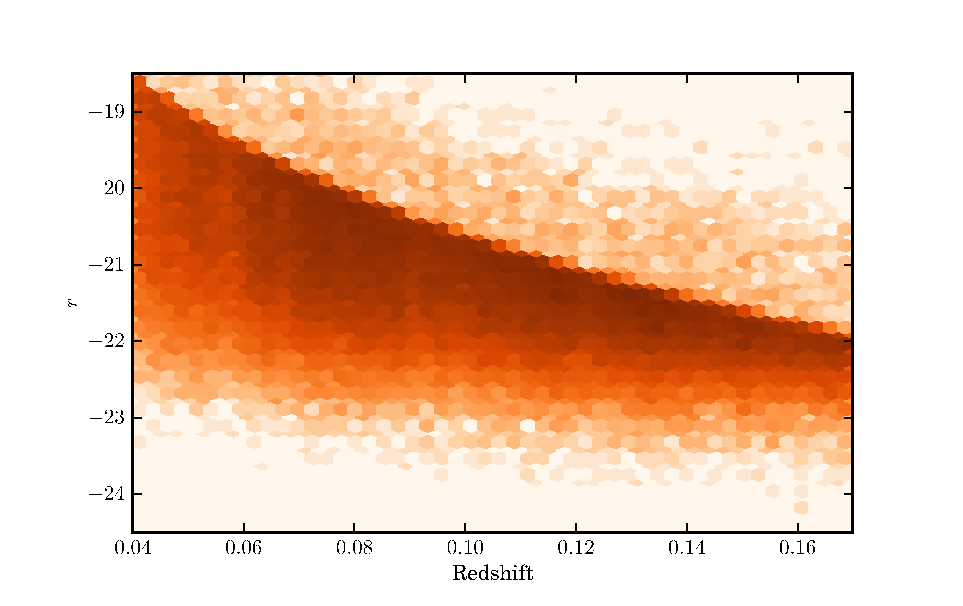
\includegraphics{figuras/completeness-volume.eps}
	\caption[Magnitude $M_r$ em função do {\em redshift}.]
	{Magnitude $M_r$ em função do {\em redshift} para a amostra \starlightUV. A
	cor dos bins hexagonais indica a densidade de pontos.}
	\label{fig:CompletezaRedshiftMag}
\end{figure}

\begin{figure}
	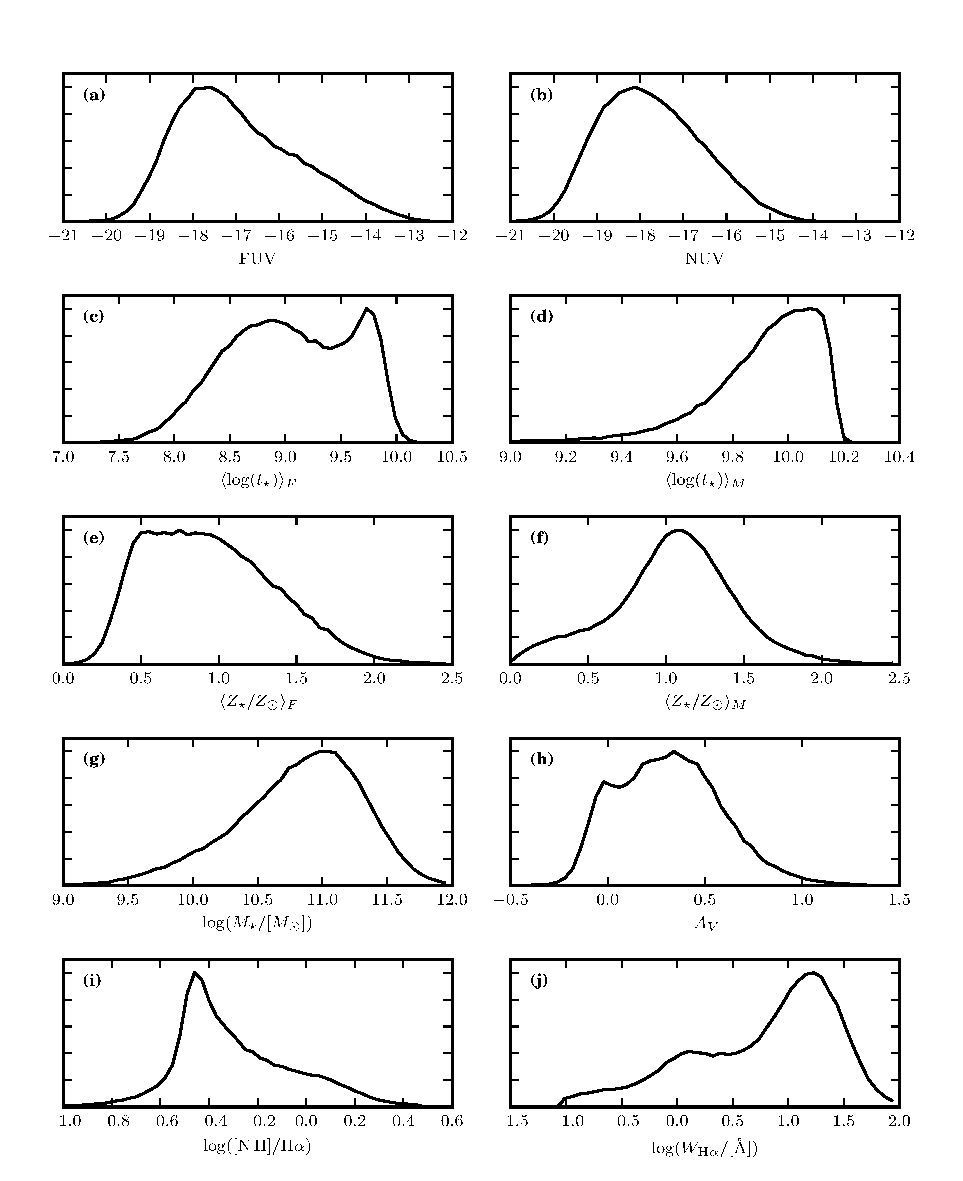
\includegraphics{figuras/histogram-sample.eps}
	\caption[Histogramas das medidas da amostra \starlightUV.]
	{Histogramas das medidas da amostra \starlightUV.}
	\label{fig:HistogramasAmostra}
\end{figure}

Resumindo, a amostra \starlightUV contém os objetos do AIS com fotometria NUV
definida, limitada em {\em redshifts} entre $0,04$ e $0,17$, e com magnitude
aparente $r$ menor que $17,77$, num total de $130\,362$ galáxias.


%% End of this chapter
